\chapter{Results and Discussion}\label{res_and_dis}\label{res_and_dis_ch}

The data collected was described in the previous Chapter, in Figure \ref{data_snip} we see a small snippet of the actual data collected. The whole data set and code for analysis can be found in Appendix \ref{ex_data_appendix} and \ref{data_anal_code}. 

\begin{figure}[]
    \centering
    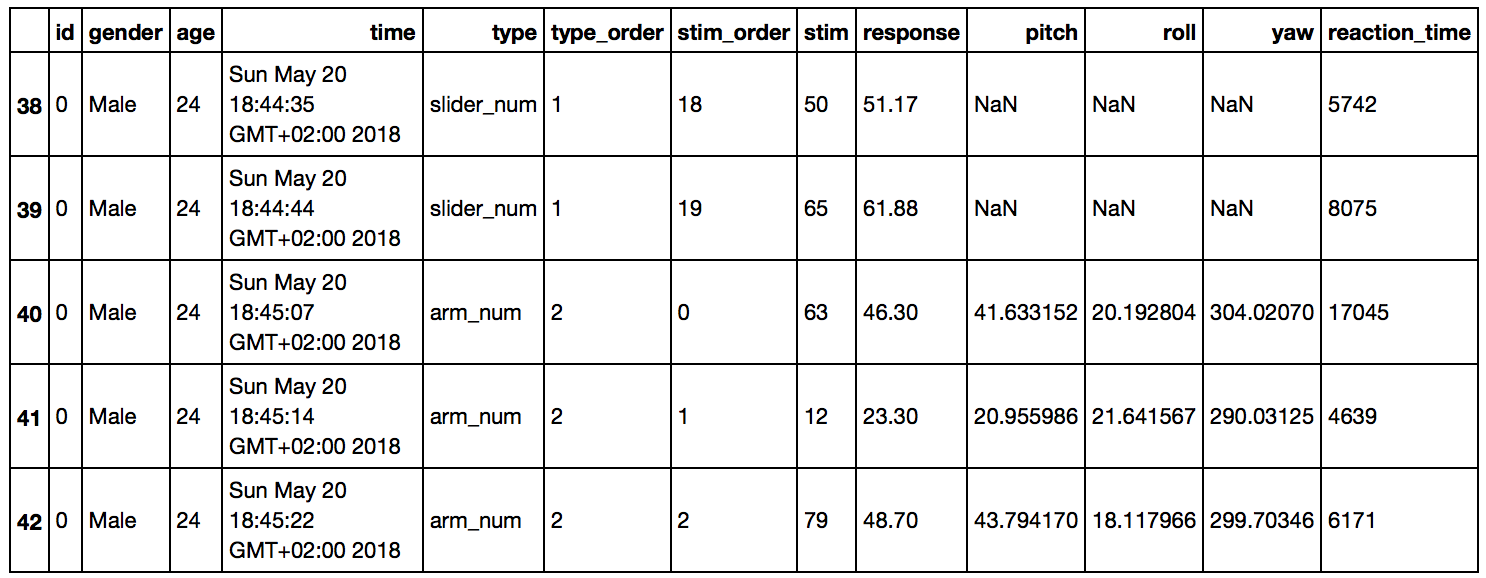
\includegraphics[width=1.2\textwidth]{figures/dataExample.png}
    \caption{Snippet of the collected data}
    \label{data_snip}
\end{figure}

In the work of Matejka et al.\cite{grey} they define any response with an error greater than half the scale to an outlier, debating that an response this far from the stimuli must be seen as a human error. Using the same argument we will remove any data point where the difference between the stimuli and response was greater than half the scale. With the grey scale exercises 50 shades of greys where shown, with a corresponding value from 0 (pure white) to 49 (pure black), therefore we will remove any data point with a difference between stimuli and response that is more than 25. Likewise with the number scale exercises where the scale is from 0 to 100 any data point with a difference between the stimuli and response greater than 50 is removed. This results in the removal of four data points, which can be seen in Figure \ref{outliers}. 

\begin{figure}[]
    \centering
    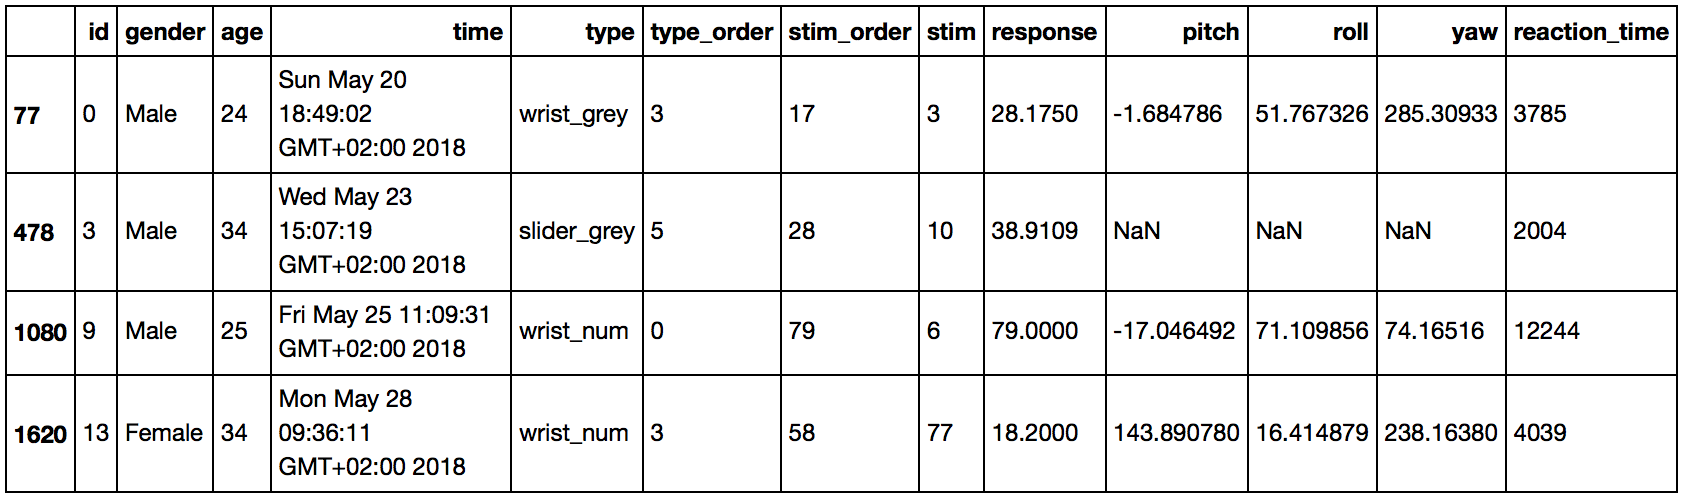
\includegraphics[width=1.2\textwidth]{figures/outliers.png}
    \caption{Four outliers that was removed from the data set}
    \label{outliers}
\end{figure}

It seems reasonable to remove these four data points, but another approach is visual inspection of the data. This can be done by plotting each participants response over stimuli for each exercise, in Figure \ref{visual_out} we the result of this for the slider on grey scale exercise, the plot has been divided into four plots with six participants on each. It then becomes easy to see by looking at each line if a point should be considered an outlier. If a line is fairly straight, but a single point is way off it can be considered an outlier, but if a line is fluctuating a lot, then it is more likely that the participant just wasn't very consistent, and therefore the a point on that line can't be considered an outlier. If we look to the lower right plot in Figure \ref{visual_out} an follow the orange line, we see that it is fairly straight, with the one exception at about (28, 12), since this is a single point that is way out line, this could be considered an outlier that must be due to user error. While this method can be effective at removing outliers, it can't be known for curtain if these point in fact are outliers, therefore this method has been discarded. The plots for the other exercises can be found in Appendix \ref{plots_appendix}.

\begin{figure}[]
    \centering
    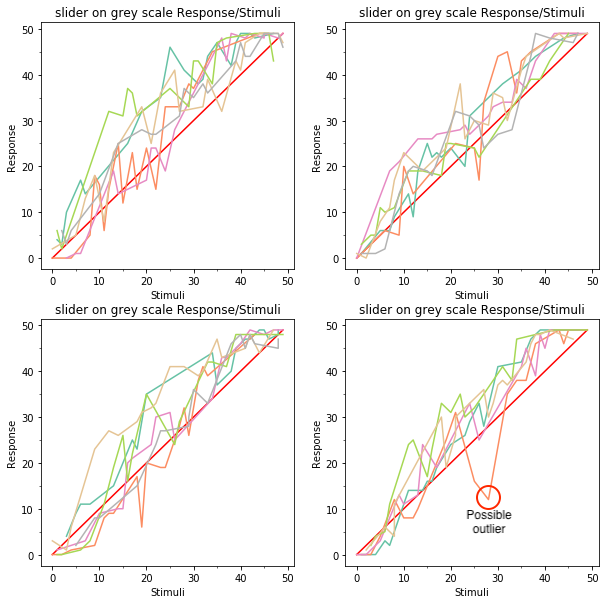
\includegraphics[width=0.75\textwidth]{figures/visual_out0.png}
    \caption{Visualization of outliers for the slider on grey scale exercise. Each line correspond to the response from a single participant. The red diagonal would be a perfect response}
    \label{visual_out}
\end{figure}

In order to compare the wristband to the digital VAS we will look into how they performed in two aspects, one is the accuracy which will be greatly investigated as this is the most important aspect to validate the use ability of the wristband. Beside the accuracy a short analysis of the task completion time of the different methods will be discussed.

\section{Accuracy}
In this experiment error is measured as the absolute difference between the stimuli and response, the lower the error the better the accuracy. Beside the error we will look into the the distribution and variance in order to describe the accuracy and compare it between the input methods. 


\subsection{Distribution and Scatters of Stimuli and Responses}
Looking at the distribution of stimuli and responses will reveal if there is any bias using any of the input methods. Since the stimuli was evenly distributed we would expect to see the same of the responses if they don't have any bias, in the following Figures the expected amount of is marked with a red line. A scatter plot of response over stimuli will visualize the errors, a perfect response will fall along the diagonal (marked with a red line), the closer the scatter is to the diagonal the smaller errors will be. We see both the distributions and scatter plots of stimuli and responses for each exercise in Figure \ref{dist_scatter1}, \ref{dist_scatter2}, \ref{dist_scatter3}, \ref{dist_scatter4}, \ref{dist_scatter5} and \ref{dist_scatter6}.


\begin{figure}[p]
    \centering
    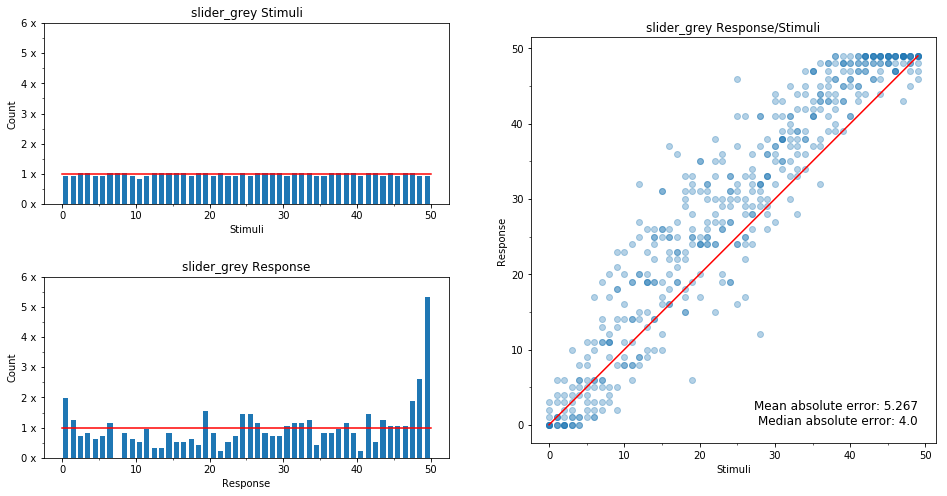
\includegraphics[width=1.2\textwidth]{figures/dist_scatter1.png}
    \caption{Distributions and scatter plot of stimuli and responses for slider on grey scale}
    \label{dist_scatter1}
\end{figure}

\begin{figure}[p]
    \centering
    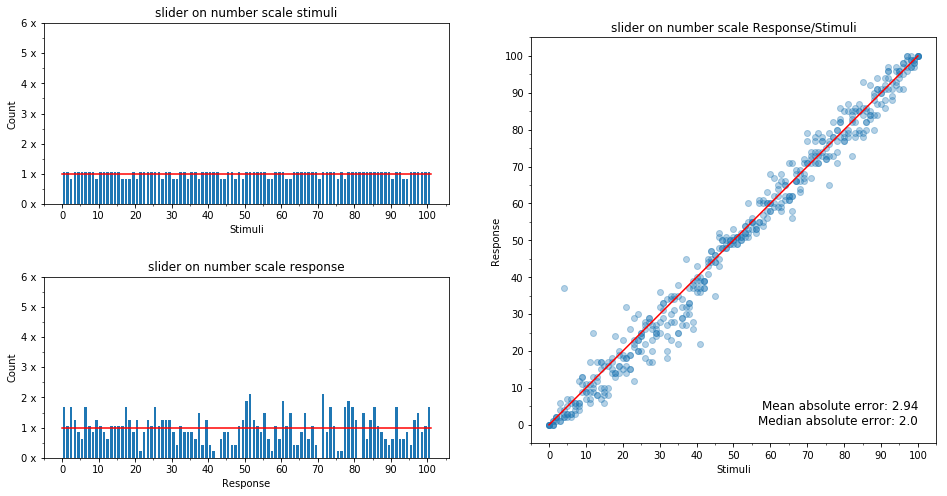
\includegraphics[width=1.2\textwidth]{figures/dist_scatter2.png}
    \caption{Distributions and scatter plot of stimuli and responses for slider on number scale}
    \label{dist_scatter2}
\end{figure}

\begin{figure}[p]
    \centering
    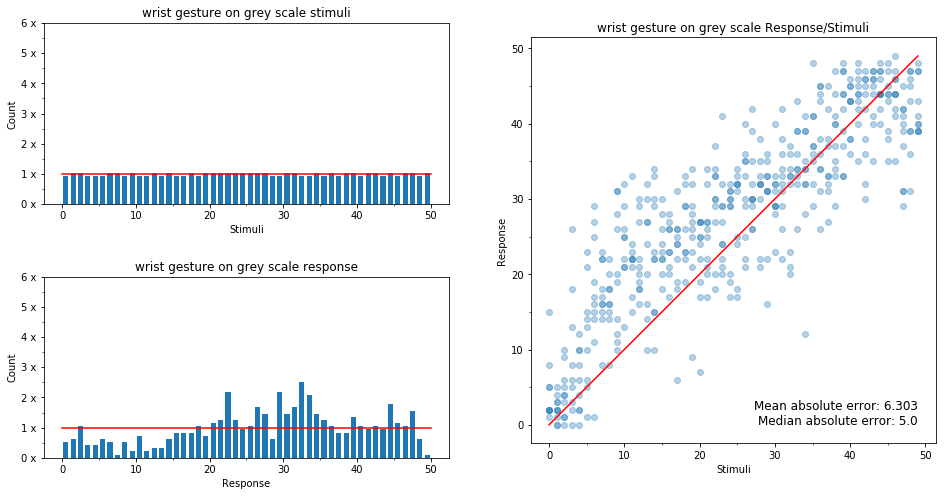
\includegraphics[width=1.2\textwidth]{figures/dist_scatter3.png}
    \caption{Distributions and scatter plot of stimuli and responses for wrist gesture on grey scale}
    \label{dist_scatter3}
\end{figure}

\begin{figure}[p]
    \centering
    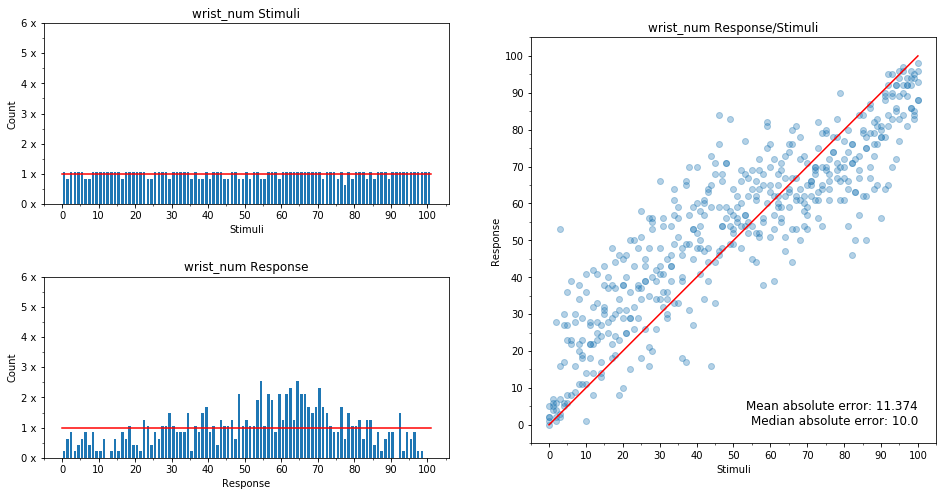
\includegraphics[width=1.2\textwidth]{figures/dist_scatter4.png}
    \caption{Distributions and scatter plot of stimuli and responses for wrist gesture on number scale}
    \label{dist_scatter4}
\end{figure}

\begin{figure}[p]
    \centering
    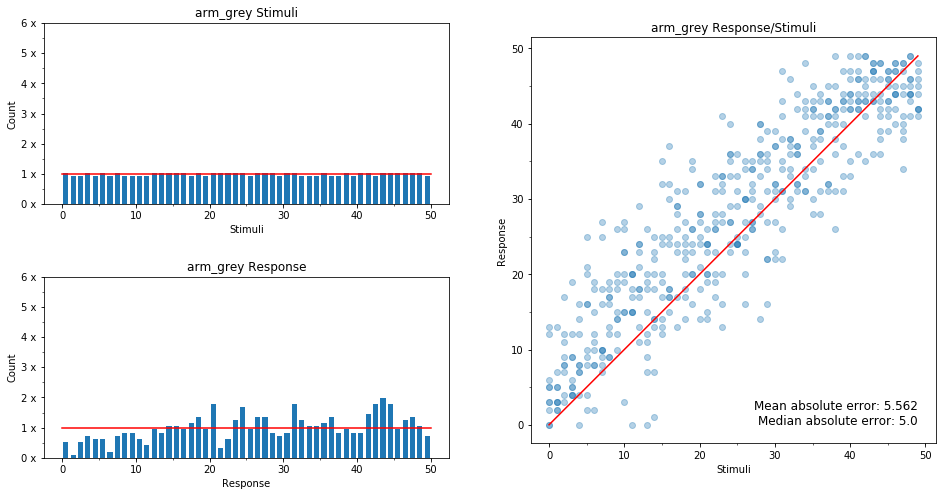
\includegraphics[width=1.2\textwidth]{figures/dist_scatter5.png}
    \caption{Distributions and scatter plot of stimuli and responses for arm gesture on grey scale}
    \label{dist_scatter5}
\end{figure}

\begin{figure}[p]
    \centering
    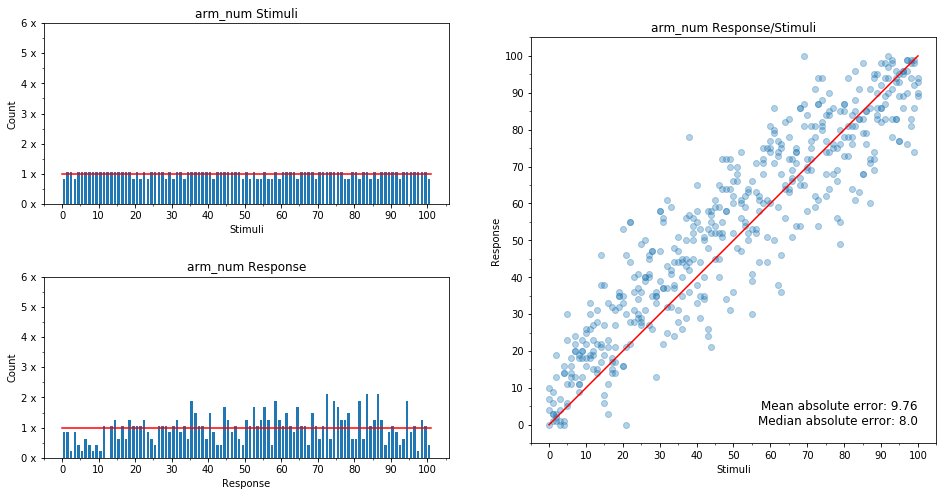
\includegraphics[width=1.2\textwidth]{figures/dist_scatter6.png}
    \caption{Distributions and scatter plot of stimuli and responses for arm gesture on number scale}
    \label{dist_scatter6}
\end{figure}

First lets investigate the distributions of stimuli and responses. First of all we see that the stimuli is evenly distributed between either 0-49 for the grey scale exercises or 0-100 for the number scale exercises, this of course is no surprise since the experiment was designed this way. We do notice that there is a little unevenness in the stimuli distribution, this is due to that each exercise had 24 participants that each performed 20 trials for a total of 480 trials. Neither 50 nor 101 is evenly dividable by this, resulting in a few stimuli being shown one time less than the others. The four outliers removed also influence this, but the overall distribution is as close to even as possible. With the distributions of the responses we don't see a perfect distribution, e.i. completely bias less, but neither do we see a largely skewed distribution meaning there isn't a strong bias. That said there are some interesting observations.

In Matejka et al.\cite{grey} work they find that when using a slider similar to the one used in this experiment, that there was a bias towards the two extremes (min and max) and the middle. In Figure \ref{dist_scatter1} we see a similar bias towards the extremes, and arguably towards the middle, although not as strong a bias as Matejka et al.'s results. They explain that the bias observed was due to the use of a slider (easy for humans to find the middle, and we tend to choose the extremes). But the distribution seen in Figure \ref{dist_scatter2} doesn't show any strong bias, since the only difference of these two exercises is the stimuli (shades of grey vs integers) then these results suggest that the bias observed in both Figure \ref{dist_scatter1} and observed by Matejka et al. is in fact not caused by the slider, but caused by the shades of grey. Looking at the shades of grey in Figure \ref{50shades} it becomes quite apparent, since it is almost impossible to differentiate pure black from the darkest shades. It is a bit easier to tell pure white apart from the light shades, this also explains why the bias toward zero is less significant. Dam-Jensen\cite{dam} found in his results that participants where only able to differentiate around 11 shades of grey, this again explain why the darker shades of grey get registered as pure black by the participants.

In Figure \ref{dist_scatter3} and \ref{dist_scatter4} we see greater amount of responses around the 32 and 65 mark respectively. We will come back to this observation soon.

Looking at the scatter plots we see can see the errors. First of all it is quite clear that the slider on number scale exercise outperforms all of the others, the scatter is very close to the diagonal. The other scatters also show a clear correlation around the diagonal, but not as close to it. In Figure \ref{dist_scatter3} and \ref{dist_scatter4} we see a very interesting observation. Looking at the scatters we see that there is a trend, with stimuli at the lower half of the scale the responses are to high and with stimuli in the upper half responses are to low. This is especially clear in Figure \ref{dist_scatter4}. It seems that there is a turning point at approximately 32 and 65 for wrist gesture on grey scale and wrist gesture on number scale respectively. These turning points are the same as we observed earlier in the distributions. A reasonable explanation for this observation can be found in biology, when investigating the wrist gesture (Figure \ref{roll}) it becomes quite apparent, because of the bone structure in the lower arm (as seen in Figure \ref{bone}) the gesture isn't linear. In the starting position of the gesture the bones are crossed and in the vertical position the bones are parallel. Since the bones aren't the same size and aren't straight this movement becomes non linear, meaning that the amount of movement required to turn the wrist from the starting position till about the halfway point is much greater than the movement needed to turn the wrist from the halfway point to the vertical position. In other words, we have a finer adjustment for the first half of the rotation than we do for the last half. It is plausible that a mathematical model could be created to compensate for this, thus improving this method, but that is beyond the scope of this thesis.

\begin{figure}[h!]
    \centering
    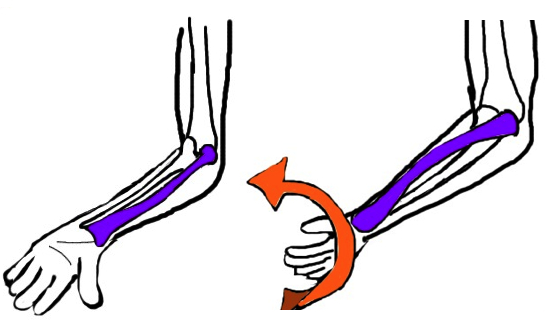
\includegraphics[width=0.5\textwidth]{figures/bone.png}
    \caption{Bone Structure of Lower Arm\cite{bone}}
    \label{bone}
\end{figure}

In Table \ref{abs_error} we see the mean, median and scaled absolute error for each exercise, these are the same values as displayed on the scatter plots. We also see see the amount of data points within $\pm$1 and $\pm$2 on a 0-10 scale, more on this later. The mean and median absolute errors are calculated across all trials for each exercise. The scaled values is the value mapped to a 0-10 scale, this is simply achieved by dividing the value by either 4.9 or 10 respectively for grey scale and number scale exercises. We see that for all exercises that the mean and median absolute error is relatively low, when scaled they are all within close to one, meaning on a 0-10 scale the responses fall close to being withing $\pm$1 of the stimuli, of course the exception being the slider on number scale which performs even better than the others.

% Please add the following required packages to your document preamble:
% \usepackage{graphicx}
\begin{table}[p]
\centering
\resizebox{\textwidth}{!}{%
\begin{tabular}{rcccccc}
 & \begin{tabular}[c]{@{}c@{}}Mean \\ abs. error\end{tabular} & \begin{tabular}[c]{@{}c@{}}Median \\ abs. error\end{tabular} & \begin{tabular}[c]{@{}c@{}}Scaled mean \\ abs. error\end{tabular} & \begin{tabular}[c]{@{}c@{}}Scaled median \\ abs. error\end{tabular} & \begin{tabular}[c]{@{}c@{}}Points\\ within $\pm$1\end{tabular} & \begin{tabular}[c]{@{}c@{}}Points\\ within $\pm$2\end{tabular} \\ \cline{2-7} 
\multicolumn{1}{r|}{slider on grey scale} & \multicolumn{1}{c|}{5.267} & \multicolumn{1}{c|}{4.0} & \multicolumn{1}{c|}{1.075} & \multicolumn{1}{c|}{0.8} & \multicolumn{1}{c|}{51.98\%} & \multicolumn{1}{c|}{79.96\%} \\ \cline{2-7} 
\multicolumn{1}{r|}{slider on number scale} & \multicolumn{1}{c|}{2.940} & \multicolumn{1}{c|}{2.0} & \multicolumn{1}{c|}{0.294} & \multicolumn{1}{c|}{0.2} & \multicolumn{1}{c|}{96.04\%} & \multicolumn{1}{c|}{99.58\%} \\ \cline{2-7} 
\multicolumn{1}{r|}{wrist gesture on grey scale} & \multicolumn{1}{c|}{6.303} & \multicolumn{1}{c|}{5.0} & \multicolumn{1}{c|}{1.286} & \multicolumn{1}{c|}{1.0} & \multicolumn{1}{c|}{43.22\%} & \multicolumn{1}{c|}{72.03\%} \\ \cline{2-7} 
\multicolumn{1}{r|}{wrist gesture on number scale} & \multicolumn{1}{c|}{11.374} & \multicolumn{1}{c|}{10.0} & \multicolumn{1}{c|}{1.137} & \multicolumn{1}{c|}{1.0} & \multicolumn{1}{c|}{48.54\%} & \multicolumn{1}{c|}{79.29\%} \\ \cline{2-7} 
\multicolumn{1}{r|}{arm gesture on grey scale} & \multicolumn{1}{c|}{5.563} & \multicolumn{1}{c|}{5.0} & \multicolumn{1}{c|}{1.135} & \multicolumn{1}{c|}{1.0} & \multicolumn{1}{c|}{48.54\%} & \multicolumn{1}{c|}{77.92\%} \\ \cline{2-7} 
\multicolumn{1}{r|}{arm gesture on number scale} & \multicolumn{1}{c|}{9.760} & \multicolumn{1}{c|}{8.0} & \multicolumn{1}{c|}{0.976} & \multicolumn{1}{c|}{0.8} & \multicolumn{1}{c|}{55.21\%} & \multicolumn{1}{c|}{88.33\%} \\ \cline{2-7} 
\end{tabular}%
}
\caption{Mean, median and scaled absolute error together with the percentage of points within $\pm$1 and $\pm$2 on the 0-10 scale for each exercise}
\label{abs_error}
\end{table}



To further illustrate how the point in the scatter plots fall based on the 0-10 scale we will add some colored bands to the plots, the green area is where the points fall within $\pm$1, together with the yellow area this is where the points fall within $\pm$2 on the 0-10 scale. On the plots the percentage of point that fall within each area is also displayed (this is also in Table \ref{abs_error}). This is seen in Figure \ref{scatter_color1}, \ref{scatter_color2} and \ref{scatter_color3}. We see that with the exeption of slider on number scale that all the other exercises performed about the same, with arm gesture on number scale performing just a bit better than the other (with the exception of slider on number scale). Based on the results so far we see no significant different between the three input methods when it comes to rating shades of grey. When rating integers from 0-100 slider on number scale strongly outperforms the other two while arm gesture on number scale is slightly better than wrist gesture on number scale.

\begin{figure}[p]
    \centering
    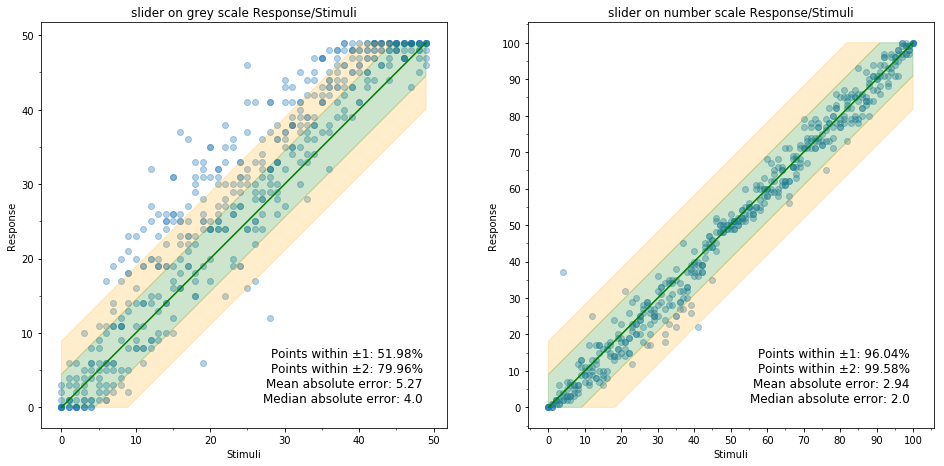
\includegraphics[width=1.15\textwidth]{figures/scatter_col1.png}
    \caption{Scatter plot with color bands for slider}
    \label{scatter_color1}
\end{figure}

\begin{figure}[p]
    \centering
    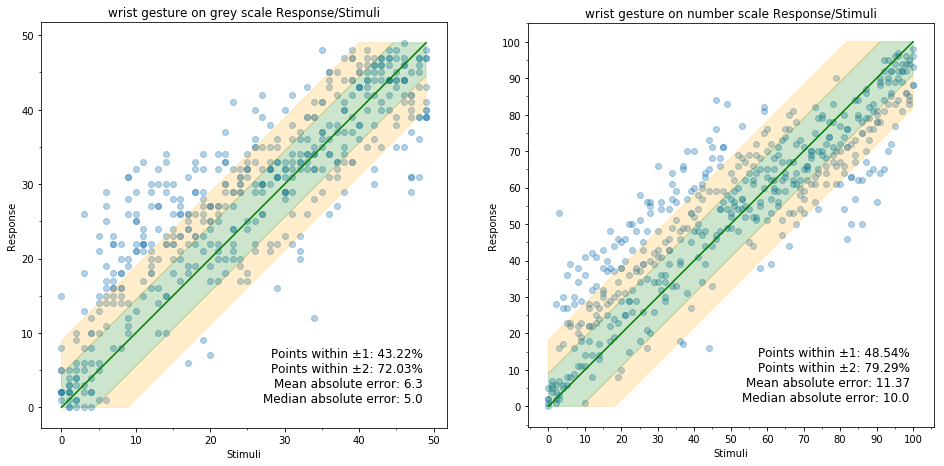
\includegraphics[width=1.15\textwidth]{figures/scatter_col2.png}
    \caption{Scatter plot with color bands for wrist gesture}
    \label{scatter_color2}
\end{figure}

\begin{figure}[p]
    \centering
    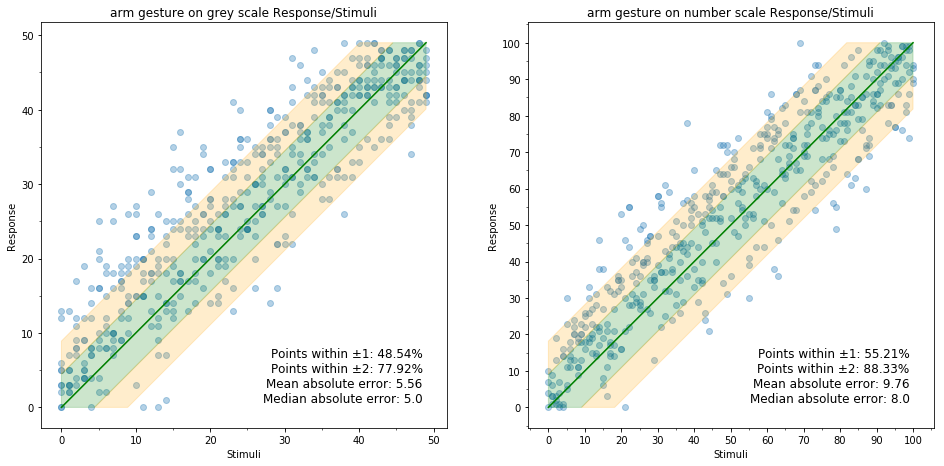
\includegraphics[width=1.15\textwidth]{figures/scatter_col3.png}
    \caption{Scatter plot with color bands for arm gesture}
    \label{scatter_color3}
\end{figure}

\subsection{Error Distribution and Variance}
To further investigate the difference in performance of the different input methods we will look into the error distribution. They will be compared visually and using t-test to see if the are statistically similar. In Figure \ref{error_dist1}, \ref{error_dist2} and \ref{error_dist3} we see the distribution of errors for the six exercises. As we would expect the errors follow a normal distribution centered around zero. Again it is clear to see that the slider on number scale performs way better than the other number scale exercises, the variance is smaller resulting in a much steeper curve meaning that the response are much closer to the stimuli. The other two number scale exercises (wrist gesture on number scale and arm gesture on number scale) seem to perform about the same. Likewise all the grey scale exercises seem to perform about the same, no clear difference in the variance or steepness of the curves.

\begin{figure}[h!]
    \centering
    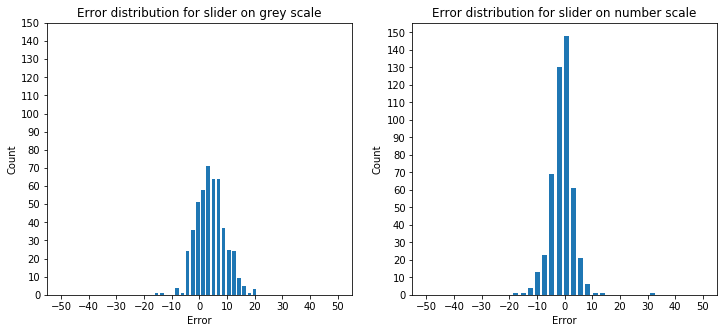
\includegraphics[width=1\textwidth]{figures/error_dist1.png}
    \caption{Error distribution for slider}
    \label{error_dist1}
\end{figure}

\begin{figure}[h!]
    \centering
    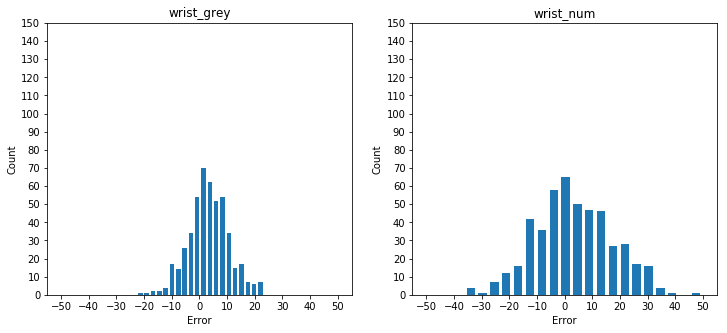
\includegraphics[width=1\textwidth]{figures/error_dist2.png}
    \caption{Error distribution for wrist gesture}
    \label{error_dist2}
\end{figure}

\begin{figure}[h!]
    \centering
    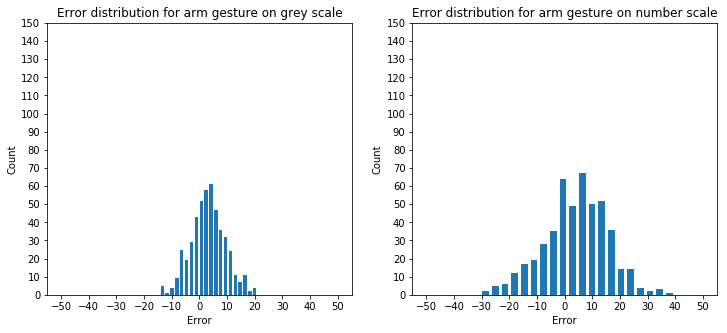
\includegraphics[width=1\textwidth]{figures/error_dist3.png}
    \caption{Error distribution for arm gesture}
    \label{error_dist3}
\end{figure}

T-test where performed between the grey scale exercises and between the number scale exercises to see if the are statistically alike. The results of the t-test can be seen in Table \ref{ttest}, for each comparison the errors from all trials of two exercises where used.

Lets start by comparing the grey scale exercises to each other. We see that wrist gesture on grey scale and arm gesture on grey scale are quite likely not to have a significant difference. From the results of comparing slider on grey scale with wrist gesture on grey scale and arm gesture on grey scale it is hard to determine weather or not they are similar. On one hand slider on grey scale and wrist gesture on grey scale is somewhat likely not to be significant different, while slider on grey scale and arm gesture on grey scale on the other hand are likely to have significant difference. These results are a bit strange, since one would assume if A and B are similar and A and C are different, then B and C must be different too, but here we see that B and C are quite similar (A being slider on grey scale, B being wrist gesture on grey scale and C being arm gesture on grey scale). That being said, the p value for wrist gesture on grey scale and arm gesture on grey scale is rather high and the calculated t-statistic is close to zero, indicating that this is the most likely case to be true out of the three.

Comparing the number scale exercises we again see that there is a clear difference between slide on number scale and the other two number scale exercises. Comparing wrist gesture on number scale and arm gesture on number scale we see that they are quite similar, meaning that statistically the change of the data being part of the same distribution is high.

Comparing grey scale exercises to number scale exercises only makes sence if comparing them with the same input method. Doing so we see the lowest p value and highest calculated t-statistic across the board when comparing slider on grey scale to slider on number scale, this is not surprising when we know how well slider on number scale performed. This indicates that there is a large difference when asked to rate shades of grey using the slider and rate integers using the slider. Both wrist and arm gesture shows to be similar when comparing the grey scale exercise to the number scale exercise, and it is quite interesting to see that wrist gesture on number scale and wrist gesture on grey scale has the highest change of being significant similar across the board. 


With these results we must conclude that the two input methods arm and wrist gesture are quite alike, while we can't say for sure if they are similar to slider when rating shades of grey we can say for curtain that arm and wrist gesture is quite different from slider when rating integers. While the t-test lest us examine the likely hood of two data sets to be similar or not, it can't tell us which performs better.



\begin{table}[]
\begin{tabular}{cccc}
\multicolumn{2}{c}{Exercises compared} & p value & Calculated t-statistic \\ \hline
\multicolumn{1}{|c|}{\begin{tabular}[c]{@{}c@{}}slider on\\ grey scale\end{tabular}} & \multicolumn{1}{c|}{\begin{tabular}[c]{@{}c@{}}wrist gesture\\ on grey scale\end{tabular}} & \multicolumn{1}{c|}{0.10045} & \multicolumn{1}{c|}{1.64426} \\ \hline
\multicolumn{1}{|c|}{\begin{tabular}[c]{@{}c@{}}slider on\\ grey scale\end{tabular}} & \multicolumn{1}{c|}{\begin{tabular}[c]{@{}c@{}}arm gesture on\\ grey scale\end{tabular}} & \multicolumn{1}{c|}{0.01598} & \multicolumn{1}{c|}{2.41378} \\ \hline
\multicolumn{1}{|c|}{\begin{tabular}[c]{@{}c@{}}wrist gesture on\\ grey scale\end{tabular}} & \multicolumn{1}{c|}{\begin{tabular}[c]{@{}c@{}}arm gesture on\\ grey scale\end{tabular}} & \multicolumn{1}{c|}{0.61034} & \multicolumn{1}{c|}{0.50976} \\ \hline
\multicolumn{1}{l}{} & \multicolumn{1}{l}{} & \multicolumn{1}{l}{} & \multicolumn{1}{l}{} \\ \hline
\multicolumn{1}{|c|}{\begin{tabular}[c]{@{}c@{}}slider on\\ number scale\end{tabular}} & \multicolumn{1}{c|}{\begin{tabular}[c]{@{}c@{}}wrist gesture on\\ number scale\end{tabular}} & \multicolumn{1}{c|}{1.29468e-10} & \multicolumn{1}{c|}{-6.49960} \\ \hline
\multicolumn{1}{|c|}{\begin{tabular}[c]{@{}c@{}}slider on\\ number scale\end{tabular}} & \multicolumn{1}{c|}{\begin{tabular}[c]{@{}c@{}}arm gesture on\\ number scale\end{tabular}} & \multicolumn{1}{c|}{9.35024e-19} & \multicolumn{1}{c|}{-9.02859} \\ \hline
\multicolumn{1}{|c|}{\begin{tabular}[c]{@{}c@{}}wrist gesture on\\ number scale\end{tabular}} & \multicolumn{1}{c|}{\begin{tabular}[c]{@{}c@{}}arm gesture on\\ number scale\end{tabular}} & \multicolumn{1}{c|}{0.39349} & \multicolumn{1}{c|}{-0.85370} \\ \hline
\multicolumn{1}{l}{} & \multicolumn{1}{l}{} & \multicolumn{1}{l}{} & \multicolumn{1}{l}{} \\ \hline
\multicolumn{1}{|c|}{\begin{tabular}[c]{@{}c@{}}slider on\\ grey scale\end{tabular}} & \multicolumn{1}{c|}{\begin{tabular}[c]{@{}c@{}}slider on\\ number scale\end{tabular}} & \multicolumn{1}{c|}{6.82003e-55} & \multicolumn{1}{c|}{16.65620} \\ \hline
\multicolumn{1}{|c|}{\begin{tabular}[c]{@{}c@{}}wrist gesture\\ on grey scale\end{tabular}} & \multicolumn{1}{c|}{\begin{tabular}[c]{@{}c@{}}wrist gesture on\\ number scale\end{tabular}} & \multicolumn{1}{c|}{0.93712} & \multicolumn{1}{c|}{0.07892} \\ \hline
\multicolumn{1}{|c|}{\begin{tabular}[c]{@{}c@{}}arm gesture on\\ grey scale\end{tabular}} & \multicolumn{1}{c|}{\begin{tabular}[c]{@{}c@{}}arm gesture on\\ number scale\end{tabular}} & \multicolumn{1}{c|}{0.14421} & \multicolumn{1}{c|}{-1.46148} \\ \hline
\end{tabular}
\caption{T-test between exercises}
\label{ttest}
\end{table}

Summarizing on the accuracy performance of the three input methods it is quite clear when it comes to rating integers that the slider outperforms both arm and wrist gesture. When it comes to rating shades of grey there seems to be no clear significant difference between the three inputs methods. And with the input methods arm and wrist gesture there doesn't seem to be a significant difference in rating shades of grey to rating integers.

\section{Task Completion Time}
The task completion time for each trial was recorded, this was the time span from the stimuli was showed to the participant registered the data. A short analysis based on the results for all the trials showed that there were no significant difference between the six exercises as shown in Table \ref{reaction_time}. There is only a little more than a second difference between the mean task completion time of the fastest and slowest exercises. Because of this no further investigation of the task completion time was conducted. The results mean that it doesn't take a significantly longer time to use the wristband than to use the slider, keep in mind that the task completion time was recorded from when stimuli was showed on screen until the participant pressed the submit button. For real life use this gives the wristband a significant advantage, since it wouldn't take much longer to use the wristband in real life than it did in the experiment, but if one where to use a digital VAS on a smartwatch the person would first have to activate the smartwatch and go through the interactions required to input the value This would involve more steps than was present in the experiment, meaning a longer total interaction time.

\begin{table}[]
\centering
\begin{tabular}{rccc}
\multicolumn{1}{c}{} & Mean & Median & \begin{tabular}[c]{@{}c@{}}Standard\\ deviation\end{tabular} \\ \cline{2-4} 
\multicolumn{1}{r|}{slider on grey scale} & \multicolumn{1}{c|}{3.589} & \multicolumn{1}{c|}{2.672} & \multicolumn{1}{c|}{2.981} \\ \cline{2-4} 
\multicolumn{1}{r|}{slider on number scale} & \multicolumn{1}{c|}{4.552} & \multicolumn{1}{c|}{3.942} & \multicolumn{1}{c|}{2.436} \\ \cline{2-4} 
\multicolumn{1}{r|}{wrist gesture on grey scale} & \multicolumn{1}{c|}{4.089} & \multicolumn{1}{c|}{3.195} & \multicolumn{1}{c|}{2.588} \\ \cline{2-4} 
\multicolumn{1}{r|}{wrist gesture on number scale} & \multicolumn{1}{c|}{4.376} & \multicolumn{1}{c|}{3.614} & \multicolumn{1}{c|}{2.553} \\ \cline{2-4} 
\multicolumn{1}{r|}{arm gesture on grey scale} & \multicolumn{1}{c|}{4.338} & \multicolumn{1}{c|}{3.563} & \multicolumn{1}{c|}{2.522} \\ \cline{2-4} 
\multicolumn{1}{r|}{arm gesture on number scale} & \multicolumn{1}{c|}{4.618} & \multicolumn{1}{c|}{3.823} & \multicolumn{1}{c|}{2.633} \\ \cline{2-4} 
\end{tabular}
\caption{Task completion time (seconds) for each exercise. The time from stimuli being shown until data was registered by the participants in each trial}
\label{reaction_time}
\end{table}



\section{Post Experiment Survey}
After the experiment the participants were asked to fill in a survey, the full survey and all the answers can be found in Appendix \ref{survey}. Unfortunately an unknown error occurred while collecting the answers, resulting in three lost answers. This section will show the results of the most relevant questions.

Given the option between the arm and wrist gesture method the participants where asked which method they preferred, which they felt was more accurate and which they felt was most comfortable. For each question they were also given the option to answer that they felt the same for both methods. The results can be seen in Table \ref{arm_vs_wrist}. Among the participants that preferred the arm gesture method they the common answer to why was that the greater range of motion allowed them to have higher precision. For the participant preferring the wrist gesture the most common reason was that it was more comfortable. For the participant that felt that the arm gesture method was more accurate their reason was that it had more precision, making it easier to make small adjustment. The two participants that felt the wrist gesture was more accurate said that they just felt like it. One participant that felt the methods to be equally accurate explained that the task felt difficult in both cases, but with practice and feedback that one could become accurate when using either method. The many participants that felt that the wrist gesture method was more comfortable explained that it was less hassle, less awkward movement and that they didn't get tired. Among the participant rating the two method equally comfortable their comments was that neither of the methods were uncomfortable to use. 


\begin{table}[h!]
\centering
\begin{tabular}{rccc}
\multicolumn{1}{c}{} & arm gesture & wrist gesture & equal \\ \cline{2-4} 
\multicolumn{1}{r|}{Preferred} & \multicolumn{1}{c|}{38.1\%} & \multicolumn{1}{c|}{42.9\%} & \multicolumn{1}{c|}{19\%} \\ \cline{2-4} 
\multicolumn{1}{r|}{Accurate} & \multicolumn{1}{c|}{81\%} & \multicolumn{1}{c|}{9.5\%} & \multicolumn{1}{c|}{9.5\%} \\ \cline{2-4} 
\multicolumn{1}{r|}{Comfort} & \multicolumn{1}{c|}{9.5\%} & \multicolumn{1}{c|}{61.9\%} & \multicolumn{1}{c|}{28.6\%} \\ \cline{2-4} 
\end{tabular}
\caption{Distribution of Answers about arm gesture vs wrist gesture (Appendix \ref{survey})}
\label{arm_vs_wrist}
\end{table}

The participants was asked if they had any prior experience using any kind of wearable devices, and with which devices (it was possible to check multiple devices). The results can be seen in Figure \ref{wearable_experience}. This showed that participants represented a good mixture of experience with wearable devices. 

\begin{figure}[]
    \centering
    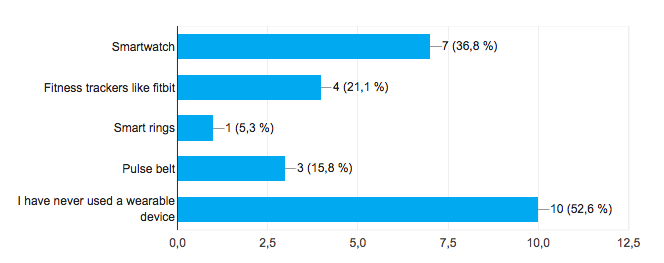
\includegraphics[width=0.8\textwidth]{figures/wearable_experience.png}
    \caption{Participants prior experience with wearable devices}
    \label{wearable_experience}
\end{figure}

Lastly the participant had a use case explained, where the had to imagine that they suffered from migraines and that their doctor had asked them to log whenever they had a headache and how severe it was. They where then presented with five different methods to log the headaches (which was described in detail) pen and paper, app on smartphone, app on smartwatch, the arm gesture method or the wrist gesture method. They where then asked to order all the method from most preferred to least preferred, the result can be seen in Figure \ref{preferred_method}. The results clearly show that the participants mostly preferred the wristband over the other methods, with pen and paper being the most disliked method. This question should only be seen as an indication, the question required the participants to think of a complex use case and make decisions on things where they probably don't have every piece of information to in order to take an informed decision. That being said the results shows promise for wristband device using the arm and wrist gestures.

\begin{figure}[]
    \centering
    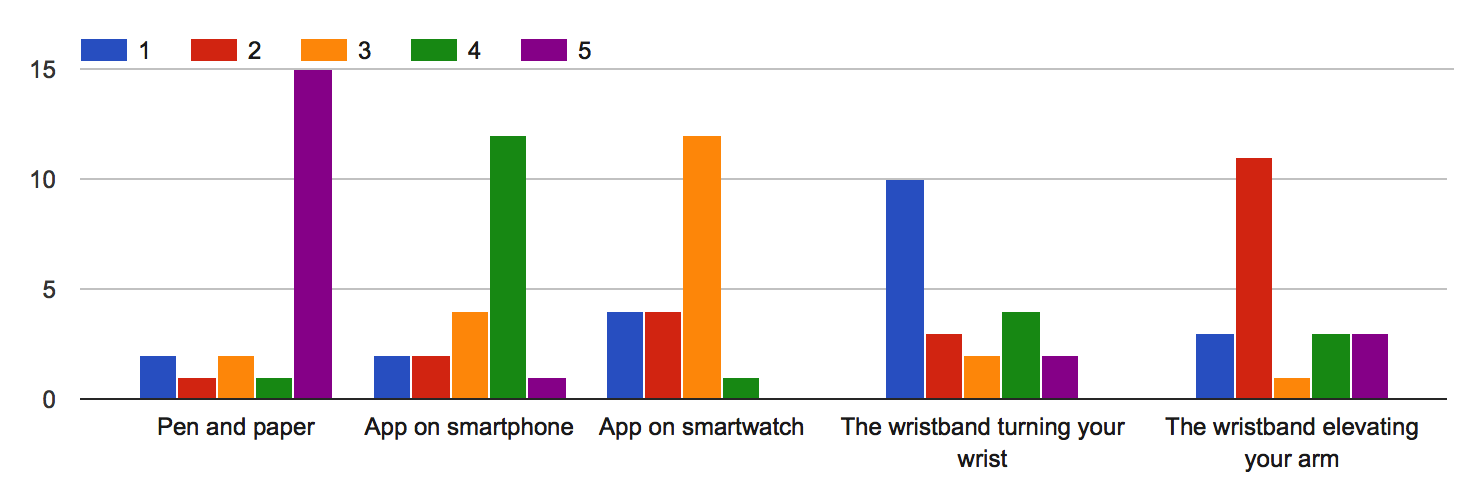
\includegraphics[width=1\textwidth]{figures/preferred_method.png}
    \caption{Rating of preferred method (1 is most preferred, 5 is least preferred)}
    \label{preferred_method}
\end{figure}

Based on all of the results, both from the experiment and the survey, is shows great promise for a use case for the wristband. It was shown that the performance of the wristband did just as good for rating shades of grey which argues it would perform well for recording  psychological events, where their isn't a specific value to record, but instead what the user feels. The arm and wrist gesture methods where shown to perform about the same, therefore either could be recommended. Based on the survey it seems to be a trade off between the feeling of accuracy and comfort, but since it has been shown that their isn't a significant difference in accuracy the wrist gesture method would be preferred to achieve a higher level of comfort.